\chapter{Background and Related Technologies}
\label{chap:background}

The Keystone framework is founded on the RISC-V instruction set architecture (ISA), which provides a compelling platform for secure system design due to its open specification and extensible modularity~\cite{lee2019keystone,dayeol2019keystone}. Unlike traditional ISAs governed by proprietary vendors, RISC-V fosters a collaborative ecosystem that supports community-driven enhancements and custom extensions. This openness uniquely positions RISC-V as a prime candidate for trusted computing research and development~\cite{Survey2023}. Furthermore, its well-defined privilege model facilitates the construction of robust isolation mechanisms, which are essential for implementing Trusted Execution Environments (TEEs).\footnote{For an in-depth exposition of RISC-V privilege modes and PMP, see the RISC-V Privilege Specification v1.10~\cite{keystone2025how}.}

RISC-V specifies three hierarchical privilege levels: user mode (U-mode), supervisor mode (S-mode), and machine mode (M-mode). M-mode operates with the highest privilege and possesses unrestricted access to hardware resources, managing critical functions such as interrupt handling, exception processing, and physical memory protection~\cite{lee2019keystone}. Keystone capitalizes on this privilege hierarchy by situating its Security Monitor (SM)—the core Trusted Computing Base (TCB)—within M-mode. The SM is responsible for managing enclaves, enforcing strict memory isolation, and mediating access to sensitive operations. By anchoring the TCB at this highest privilege level, Keystone minimizes the trusted surface exposed to potential attackers.

A key hardware feature leveraged by Keystone is the Physical Memory Protection (PMP) unit, introduced in the RISC-V Privilege Specification v1.10. PMP empowers M-mode software to define fine-grained access permissions for physical memory regions, specifying which lower privilege levels (U and S) may read, write, or execute code therein~\cite{keystone2025how}. This hardware-enforced mechanism forms the cornerstone of Keystone’s memory isolation strategy. Each enclave is assigned a dedicated, PMP-protected memory region that remains inaccessible to the host OS or unauthorized software, guaranteeing strong confidentiality and integrity guarantees enforced at the hardware level~\cite{lee2019keystone}.

In addition to PMP, RISC-V’s flexible trap and exception handling model enables M-mode to intercept all traps while optionally delegating certain classes, such as system calls and page faults, to S-mode for efficiency~\cite{lee2019keystone}. This delegation mechanism facilitates cooperation between enclave runtimes and the host OS for memory management without compromising enclave boundaries. Keystone utilizes the RISC-V Memory Management Unit (MMU) to support private virtual address spaces per enclave, further fortified by PMP protections against unauthorized access or tampering~\cite{dayeol2019keystone}.

Notably, the Keystone Security Monitor is implemented in C using standard programming toolchains, which enhances maintainability, auditability, and formal verification potential. This contrasts with fixed-function microcode or proprietary firmware that is often opaque and difficult to analyze, thus bolstering Keystone’s transparency and security assurance~\cite{lee2019keystone}.

Together, the RISC-V privilege hierarchy, PMP, trap delegation, and extensibility create a robust substrate for implementing flexible, open, and secure TEEs. Keystone exploits these architectural advantages to deliver a customizable and transparent enclave platform aligned with the open philosophy of RISC-V~\cite{Survey2023}.

\section{Trusted Execution Environments}

Trusted Execution Environments (TEEs) are specialized hardware-assisted secure computing architectures designed to provide strong confidentiality and integrity guarantees for code and data, even in the presence of compromised system software~\cite{Survey2023,suzaki2021tsperf}. By establishing isolated execution contexts—often termed enclaves—TEEs protect sensitive computations through a combination of hardware-enforced isolation and minimal trusted software components.

A TEE effectively partitions system resources such as CPU registers, memory, and I/O peripherals, restricting access exclusively to trusted enclave applications. This isolation is enforced by the processor’s privilege levels, memory protection units, or dedicated security monitors, thereby preventing unauthorized entities—including kernel-level malware or user-space adversaries—from accessing or manipulating enclave data~\cite{brasser2019software}.

Security in TEEs hinges on minimizing the Trusted Computing Base (TCB), which encompasses all components that must be trusted for correct and secure operation. A smaller TCB reduces the risk of vulnerabilities and facilitates formal verification and security audits~\cite{lee2019keystone,Survey2023}. Modern TEEs strive to encapsulate only essential components within the TCB, balancing security with functionality.

Commercially dominant TEE solutions include Intel Software Guard Extensions (SGX) and ARM TrustZone. Intel SGX enables enclave creation at user privilege levels, employing hardware-enforced memory encryption and access controls~\cite{costan2016intel}. ARM TrustZone employs a split-world model that partitions processor execution into secure and normal worlds, with transitions mediated by secure monitor calls~\cite{yan2018trustzone}. Despite their widespread deployment, these architectures suffer from proprietary designs and limited transparency, which constrain their flexibility for academic research and system-level innovation.

In contrast, open-source TEE frameworks such as Keystone have emerged to address these limitations by leveraging the open, modular RISC-V ISA~\cite{lee2019keystone,dayeol2019keystone}. The modularity and openness of RISC-V facilitate the design of TEEs that are both highly configurable and more transparent, fostering security research and experimentation~\cite{Survey2023}. A central architectural principle of TEEs, exemplified by Keystone, is privilege separation: executing the TCB in the highest privilege mode (M-mode in RISC-V) while relegating untrusted software to lower privilege levels. This design enforces strict isolation policies, preventing untrusted software from compromising enclave security~\cite{lee2019keystone}.

By integrating privilege separation, hardware-enforced memory protections, and modular TCB design, TEEs provide a powerful framework for secure computation within adversarial environments. Keystone extends these foundational principles with openness and configurability, offering a valuable platform for both academic research and practical deployments of trusted computing technologies~\cite{suzaki2021tsperf}.


\section{Keystone Enclave Architecture}

Keystone is an open-source Trusted Execution Environment (TEE) framework built on the RISC-V architecture, designed to enable customizable, lightweight, and secure enclaves suitable for both research and deployment in resource-constrained or security-critical settings \cite{dayeol2019keystone}. The framework’s modular design emphasizes a minimal Trusted Computing Base (TCB), portability across diverse RISC-V platforms, and extensibility to accommodate advanced security features, reflecting a clean and flexible architectural philosophy.

Keystone leverages the multiple privilege modes defined by the RISC-V specification—user mode (U-mode), supervisor mode (S-mode), and machine mode (M-mode)—to enforce security policies effectively. At the core of Keystone’s TCB is the Security Monitor (SM), which executes in M-mode and holds exclusive authority over enclave lifecycle management, memory protection configuration, and access control enforcement. The SM uses RISC-V’s Physical Memory Protection (PMP) mechanism to isolate enclave memory regions dynamically, ensuring strict access controls during enclave execution \cite{dayeol2019keystone}.

A typical Keystone-enabled platform comprises RISC-V cores augmented with secure boot mechanisms, trusted entropy sources, and optionally, hardware accelerators for cryptographic functions or secure I/O. Importantly, Keystone does not require hardware beyond standard RISC-V compliance and PMP support, making it adaptable to implementations ranging from FPGA prototypes to silicon SoCs \cite{dayeol2019keystone}.

Each enclave in Keystone consists of two main software components: a user-level enclave application (eapp) containing application-specific logic, and a supervisor-level runtime (RT) providing essential operating system abstractions such as exception handling, system call services, and memory management. This layered approach reduces the complexity of enclave applications and provides a trusted runtime environment isolated from the untrusted operating system and other processes \cite{dayeol2019keystone}.

The enclave lifecycle is structured into three primary phases: creation, execution, and destruction. During creation, the SM validates and locks the enclave’s memory layout—referred to as Enclave Page Memory (EPM)—with PMP to ensure confidentiality and integrity. During execution, the SM mediates context switches between the host and enclave, dynamically adjusting PMP to maintain isolation. Destruction securely erases enclave memory to prevent any residual data leakage \cite{dayeol2019keystone}. Keystone also supports optional features such as remote attestation, allowing external verifiers to authenticate enclave state prior to provisioning sensitive data, and can be extended for secure I/O and cryptographic acceleration.

\begin{figure}[htbp]
\centering
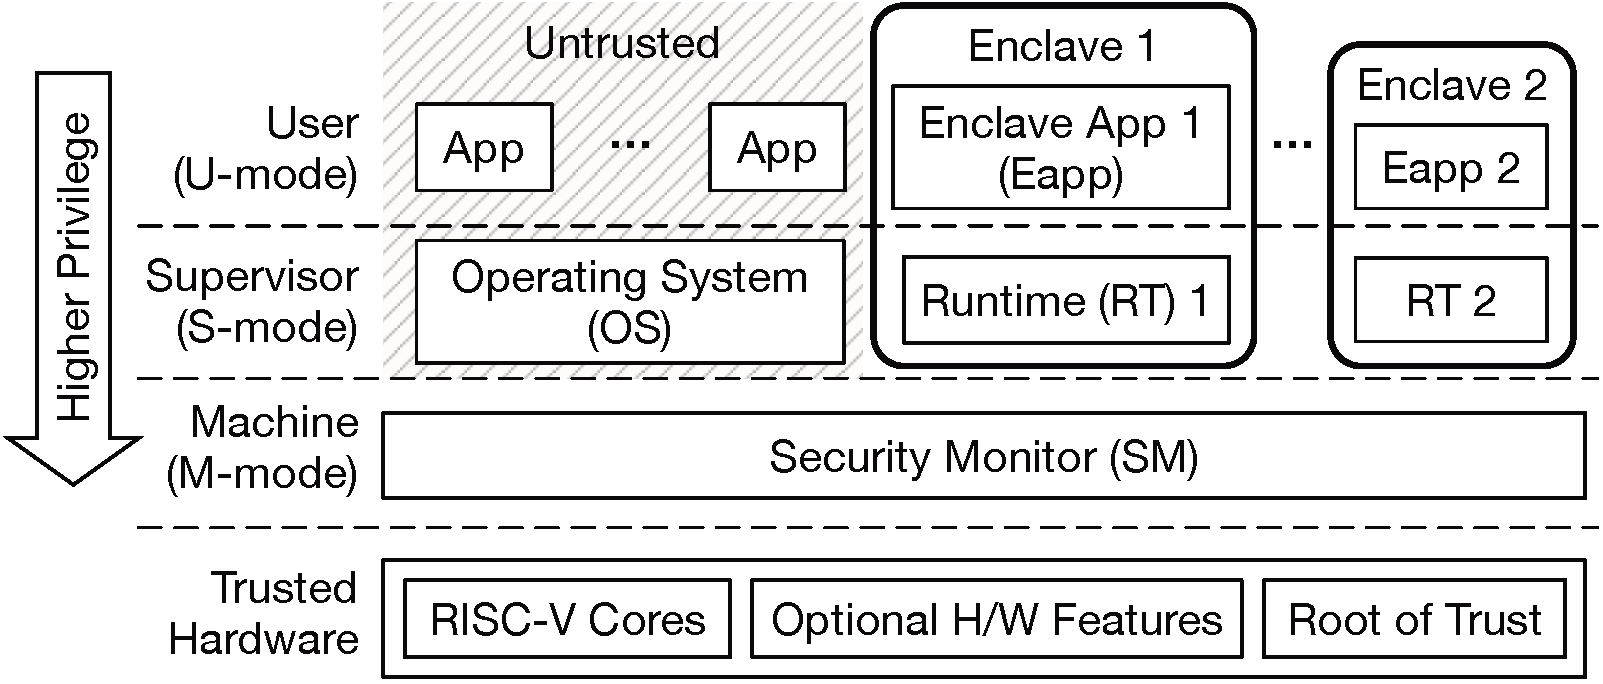
\includegraphics[width=0.9\linewidth]{figures/keystone_overview.png}
\caption{Overview of the Keystone architecture illustrating components such as the Security Monitor, enclave runtime, and the privilege hierarchy.}
\label{fig:keystone_overview}
\end{figure}

\begin{figure}[htbp]
\centering
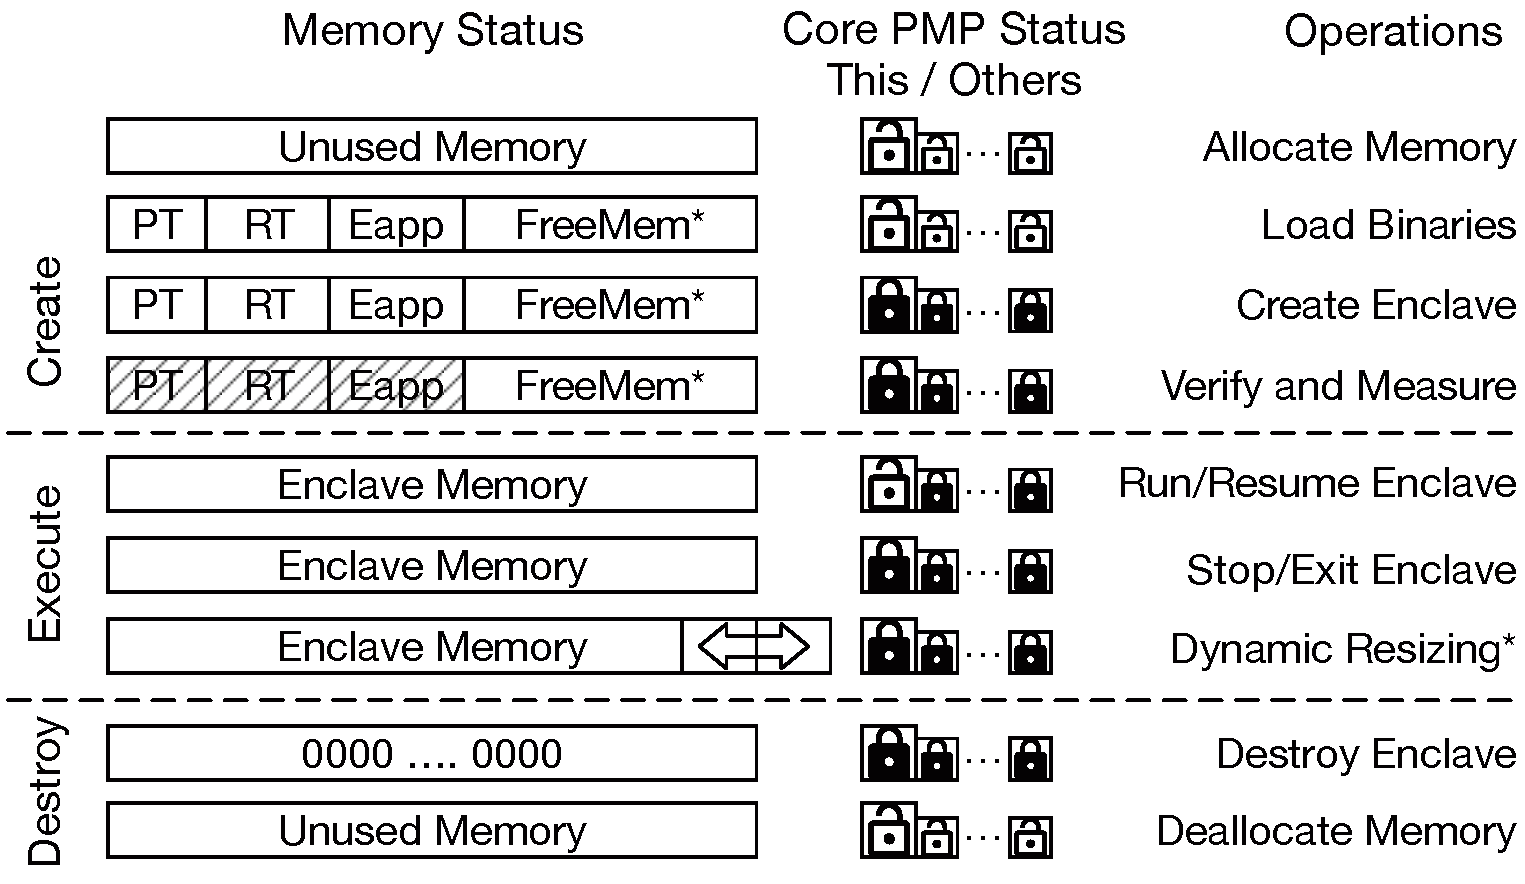
\includegraphics[width=0.9\linewidth]{figures/enclave_lifecycle.png}
\caption{Stages of a Keystone enclave lifecycle: creation, execution, and destruction.}
\label{fig:enclave_lifecycle}
\end{figure}

Keystone’s modular and open framework leverages the openness of RISC-V to provide strong security guarantees while enabling flexibility for research and customization. Its minimal TCB, modular layering (Security Monitor, runtime, eapp), and standards-compliant interfaces make it an attractive platform for developing and evaluating secure applications on modern processors \cite{dayeol2019keystone}. 
To support secure communication and attestation, Keystone enclaves can integrate modern cryptographic primitives, including emerging post-quantum schemes such as Kyber.

\section{Physical Memory Protection (PMP) in RISC-V}

\section{Post-Quantum Cryptography: Kyber Algorithm}
\label{sec:kyber}

Kyber is a post-quantum key encapsulation mechanism (KEM) designed to resist attacks from both classical and quantum adversaries. Its security is based on the hardness of the Module Learning With Errors (Module-LWE) problem, a structured lattice problem considered intractable even for quantum computers. Kyber is one of the finalists in the NIST Post-Quantum Cryptography (PQC) competition and has been selected for standardization due to its strong security and performance characteristics \cite{kyber2024}.  % [SOURCE1]

At its core, Kyber is derived from the Lyubashevsky–Peikert–Regev (LPR) encryption framework, which adapts Learning With Errors (LWE) from integer vectors to more efficient polynomial structures. Specifically, Kyber operates in the Module-LWE setting, which balances the structure of Ring-LWE with the flexibility of traditional LWE. This results in strong performance and compact key sizes while preserving security \cite{kyber2024,kyber2021}. % [SOURCE1, BLOG1]

Kyber supports three security levels:
\begin{itemize}
    \item \textbf{Kyber-512}, targeting AES-128-level security,
    \item \textbf{Kyber-768}, targeting AES-192-level security (recommended),
    \item \textbf{Kyber-1024}, targeting AES-256-level security.
\end{itemize}

\begin{table}[h]
\centering
\caption{Kyber and RSA: Key and Ciphertext Sizes (in bytes)}
\label{tab:kyber_sizes}
\begin{tabular}{|l|c|c|c|}
\hline
\textbf{Scheme} & \textbf{Private Key} & \textbf{Public Key} & \textbf{Ciphertext} \\
\hline
Kyber-512 & 1632 & 800 & 768 \\
Kyber-768 & 2400 & 1184 & 1088 \\
Kyber-1024 & 3168 & 1568 & 1568 \\
RSA-3072 & 384 & 384 & 384 \\
RSA-15360 & 1920 & 1920 & 1920 \\
\hline
\end{tabular}
\end{table}

While RSA keys are somewhat smaller, Kyber maintains significantly better security in the post-quantum context, and its keys are far more compact than those of many alternative PQC candidates such as Classic McEliece \cite{kyber2021}. % [BLOG1]

Kyber is structured as a KEM rather than a traditional public-key encryption (PKE) scheme. Internally, however, it uses a PKE system transformed into a CCA-secure KEM. The KEM exposes a simple API:
\begin{itemize}
    \item $(\mathit{pk}, \mathit{sk}) = \texttt{KeyGen}()$
    \item $(\mathit{ct}, \mathit{ss}) = \texttt{Encapsulate}(\mathit{pk})$
    \item $\mathit{ss} = \texttt{Decapsulate}(\mathit{sk}, \mathit{ct})$
\end{itemize}

The encapsulation mechanism makes Kyber especially suitable for protocols like TLS, Signal, and OpenPGP. % [BLOG1]

A simplified pedagogical version called ``Baby Kyber’’ is often used to illustrate the cryptographic structure. Baby Kyber uses polynomials over a small modulus and limited degree to show how private and public keys, as well as ciphertexts, are constructed and manipulated. Encryption relies on adding small random errors to hide the message, while decryption relies on error tolerance due to coefficient scaling. If the message polynomial is scaled appropriately, decryption can recover the original bit string by rounding \cite{kyber2021}. % [BLOG1]

In full Kyber, the parameters are chosen to ensure security and correctness:
\begin{itemize}
    \item $n = 256$: polynomial degree
    \item $k \in \{2, 3, 4\}$: number of polynomials (Kyber-512, 768, 1024)
    \item $q = 3329$: prime modulus
    \item $\eta_1, \eta_2$: bounds on error distributions
    \item $d_u, d_v$: compression factors
\end{itemize}

Kyber’s performance has been optimized for a variety of platforms. Table~\ref{tab:kyber_perf} shows benchmark results on an Intel Haswell CPU with AVX2 vectorization \cite{kyber2024}. % [SOURCE1]

\begin{table}[h]
\centering
\caption{Kyber Performance on Haswell CPU (AVX2 Optimized)}
\label{tab:kyber_perf}
\begin{tabular}{|l|c|c|c|}
\hline
\textbf{Variant} & \textbf{KeyGen (cycles)} & \textbf{Encaps (cycles)} & \textbf{Decaps (cycles)} \\
\hline
Kyber-512 & 33,856 & 45,200 & 34,572 \\
Kyber-768 & 52,732 & 67,624 & 53,156 \\
Kyber-1024 & 73,544 & 97,324 & 79,128 \\
\hline
\end{tabular}
\end{table}

Kyber also includes a variant called \texttt{Kyber-90s}, which replaces the use of SHAKE with AES-256 and SHA2 primitives, enabling further acceleration on platforms with AES instruction support \cite{kyber2024}. % [SOURCE1]

The security of Kyber ultimately reduces to the hardness of the Shortest Vector Problem (SVP) via the Module-LWE problem. Recovering a message or key requires solving an instance of SVP in a structured lattice, a task that remains intractable even with quantum resources\cite{kyber2021}. % [BLOG1]

Due to its efficient structure and compact representation, Kyber has been adopted by numerous organizations:
\begin{itemize}
    \item Cloudflare included Kyber in the CIRCL cryptographic library
    \item Amazon integrated hybrid Kyber modes into AWS KMS
    \item IBM deployed Kyber in its quantum-secure tape drive
\end{itemize} % [SOURCE1]
These deployments demonstrate Kyber’s readiness for practical applications in secure communications, data protection, and cryptographic protocols. 
The integration of Kyber into TEE frameworks like Keystone is increasingly relevant as systems must remain secure even in the presence of quantum-capable adversaries. TEEs benefit from Kyber’s compact keys and efficient operations, making it a strong candidate for enclave-based key exchange and attestation.

\section{Comparative Overview of TEE}
\label{sec:comparison_tees}

Keystone distinguishes itself from commercial Trusted Execution Environments—such as Intel SGX, ARM TrustZone, and AMD SEV—through its unique design choices, combining openness, modularity, and deep alignment with the RISC‑V ecosystem.

First and foremost, Keystone is fully open-source, enabling complete transparency and extensibility. This contrasts sharply with the proprietary nature of SGX, TrustZone, and SEV, which limits research innovation and system adaptability \cite{turn0search0}. The open stance of Keystone allows researchers to inspect, customize, and formally verify its components, significantly reducing the Trusted Computing Base (TCB) compared to monolithic Secure World kernels or hardware-bound enclaves \cite{turn0search0}.

ARM TrustZone operates using a dual-world model: a Secure World and a Normal World, switching through secure monitor calls (SMCs). While effective, this design suffers from overhead due to frequent context switching and increased TCB complexity since the Secure World often incorporates a full OS stack (e.g., OP‑TEE) \cite{turn0search0}. In contrast, Intel SGX allows enclave creation at user-level with encrypted memory regions but remains constrained by limited enclave size, single-mode operation, and dependency on Intel hardware, hindering portability and flexibility \cite{turn0search0}.

Keystone effectively synthesizes the strengths of these platforms while avoiding their limitations. It supports dynamic enclave creation spanning both user and supervisor modes, with security ensured via low-overhead Physical Memory Protection (PMP) and a lightweight, verifiable Security Monitor operating in M-mode \cite{dayeol2019keystone}. This design offers richer enclave functionality with reduced complexity.

Empirical comparisons further highlight Keystone’s competitive performance. TS‑Perf, a systematic benchmarking framework, measured execution time across SGX, TrustZone, and RISC‑V Keystone using identical binaries and workloads (e.g., internal APIs, matrix operations, memory and storage access). It reports how architectural differences manifest in performance across ecosystems \cite{turn0search5}. Broader experimental evaluations, such as those comparing SGX, SEV, and Intel TDX, emphasize their varying overheads in CPU-, memory-, and I/O-bound workloads. These comparisons underscore that Keystone—while not the fastest in all cases—offers compelling performance coupled with openness and ease of extension \cite{turn0search2,turn0search10}.

Feature-wise, trusted computing surveys place Keystone in a distinct category: unlike SGX and SEV, which emphasize encryption and hardware-rooted attestation, Keystone enables both secure and flexible enclave configurations, attested through PMP and monitor mechanisms, and retains openness—making it uniquely suitable for research-oriented and evolving hardware/software environments \cite{turn0search9}.

For these reasons, Keystone represents a promising alternative to closed-source TEEs, especially in academic and experimental contexts.


\section{Performance Challenges in Secure Execution}

Trusted Execution Environments (TEEs) introduce strong isolation guarantees that are essential for secure computation, but these guarantees often come at the cost of non-negligible performance overheads. This performance degradation arises from several sources, including architectural constraints, software abstraction layers, and platform-specific implementation trade-offs. Understanding these performance characteristics is crucial to evaluating the practical deployment of TEEs, especially in scenarios requiring low latency or high throughput.

Compute-bound workloads tend to experience the least disruption from TEE isolation mechanisms. Operations such as arithmetic computations that remain within the processor’s execution pipeline typically show minimal slowdown. Empirical studies using TS-perf and Keystone’s own benchmarking tools (e.g., CoreMark and RV8) indicate that when enclave creation and destruction costs are excluded, the performance overhead of TEEs for CPU-intensive tasks is often below 1\%, with Intel SGX, ARM TrustZone, and RISC-V Keystone all exhibiting similar behavior \cite{Suzaki2021,dayeol2019keystone}.

However, memory-bound applications face a very different scenario. Memory isolation mechanisms—particularly those involving encryption, cache partitioning, and page fault handling—can significantly impact runtime performance. For instance, in the Keystone framework, applications such as \texttt{miniz} and \texttt{aes} that utilize large memory footprints have shown over 100\% slowdown when cache partitioning is enabled, due to increased cache misses and eviction rates \cite{dayeol2019keystone}. Similarly, TS-perf benchmarks report an 11\% reduction in performance for ARM TrustZone under random memory access workloads, largely attributable to memory encryption and hierarchy constraints \cite{Suzaki2021}. SGX-based systems experience a sharp decline in performance once the enclave's memory usage exceeds the size of the Enclave Page Cache (EPC), which triggers expensive paging behavior; this trend has been documented comprehensively by SGXGauge \cite{kumar2022sgxgauge}. Scientific computing workloads running on SGX and AMD SEV platforms have demonstrated slowdown factors ranging from 1.2× up to 126×, depending on workload characteristics and hardware constraints \cite{akkram2020scientific}.

To address these performance issues, researchers have proposed alternative memory models that relax or restructure the traditional enclave-host memory boundaries. One such innovation is Elasticlave, a shared-memory model designed for enclaves that reduces isolation costs while preserving strong security properties. Elasticlave achieves an order of magnitude better performance compared to traditional spatial isolation models, with overheads as low as 10\% versus 100× to 1000× for spatially isolated configurations \cite{yu2022elasticlave}. Similarly, Eleos introduces self-paging within enclaves, allowing the enclave itself to manage virtual memory. This eliminates host OS involvement in page fault handling and mitigates context-switching and cache pollution overheads, resulting in significantly improved runtime efficiency \cite{orenbach2023eleos}. A related approach, Cerberus, applies formal methods to build a provably secure enclave memory-sharing model on Keystone. It enables safe data sharing with external components without compromising security, all while reducing redundancy and memory copying overheads \cite{lee2022cerberus}.

Input/output (I/O) operations also suffer substantial performance penalties in TEE contexts due to the need for secure copying and context switching. In Keystone, file I/O performance as measured using IOZone demonstrates a 36.2\% decrease in write throughput and a 40.9\% reduction in read throughput when compared to execution in the Rich Execution Environment (REE). Repetitive operations, such as record rewriting, exhibit even greater overhead—up to 55.1\% \cite{dayeol2019keystone}. These trends are consistent across other platforms as well; TS-perf reveals that both OP-TEE and SGX-based file operations incur high latency due to their reliance on ECALLs and limited in-enclave storage APIs \cite{Suzaki2021}.

Even basic services such as time measurement exhibit significant variability depending on how they are implemented. For example, \texttt{TEE\_GetREETime()}—which retrieves the time from the REE—requires a context switch and is consequently far slower than \texttt{TEE\_GetSystemTime()}, which accesses an enclave-resident hardware timer. The performance difference between these two methods can be as high as 30×, illustrating how even seemingly simple operations may be subject to substantial overhead within a TEE \cite{Suzaki2021}.

An additional source of performance variability lies in runtime behavior and process scheduling. Observations from TS-perf experiments showed unexpected enclave behavior such as thread migration between CPU cores and incorrect CPU utilization reporting, particularly in OP-TEE and Keystone environments. These anomalies were traced to a lack of TEE-awareness in OS-level schedulers and, in Keystone's case, bugs in the Eyrie runtime's interrupt handling mechanism \cite{Suzaki2021}.

Monitoring and profiling enclave performance in real-time remains a difficult task. TEEMon provides a lightweight performance monitoring framework designed specifically for TEE environments. Though it introduces between 5–17\% overhead, it enables continuous visibility into runtime behavior and facilitates the identification of performance bottlenecks that would otherwise be hidden \cite{krahn2020teemon}.

Finally, the cost of lifecycle operations—such as enclave initialization and teardown—should not be underestimated. In Keystone, these operations involve verifying memory integrity through hashing (e.g., SHA-3) and setting up cryptographic metadata. These steps consume between 2M–7M cycles per page for validation, and an additional 20k–30k cycles for each lifecycle event. The use of software-based cryptographic primitives amplifies these costs, though hardware acceleration could substantially mitigate them in future implementations \cite{dayeol2019keystone}.

While TEEs demonstrate excellent performance for compute-bound applications, they impose substantial overheads for workloads that are memory-intensive, I/O-heavy, or reliant on low-latency system services. These performance limitations vary across platforms and are deeply influenced by architectural decisions, memory subsystem behavior, scheduling models, and the design of enclave runtimes. As TEE adoption expands, especially in embedded and latency-sensitive environments, mitigating these performance challenges will require both architectural innovation and co-design between software and hardware components.

%\section{Post-Quantum Cryptography and Kyber}
%\section{Performance Considerations for PQC in TEEs}